\documentclass[12pt,letterpaper,answers]{exam}
%\usepackage{color}
\usepackage[usenames,dvipsnames,svgnames,table]{xcolor}
\usepackage[margin=0.9in]{geometry}
\renewcommand{\familydefault}{\sfdefault}
\usepackage{multicol}
\pagestyle{head}
\definecolor{c02}{HTML}{FFBBBB}
\definecolor{c03}{HTML}{FFDDDD}
\header{AM 108 Problem Set 05}{}{{\colorbox{c02}{\makebox[3.0cm][l]{Due Fri Mar 3}}}\\ at noon p.\thepage}
\runningheadrule
\headrule
\usepackage{diagbox}
\usepackage{graphicx} % more modern
%\usepackage{subfigure} 
\usepackage{amsmath} 
\usepackage{amssymb} 
%\usepackage{gensymb} 
%\usepackage{natbib}
\usepackage{hyperref}
%\usepackage{enumitem}
%\setlength{\parindent}{0pt}
%\usepackage{setspace}
%\pagestyle{empty}  
%\newcommand{\Sc}[0]{
%{\color{BlueViolet}\S}
%}
\usepackage{tcolorbox}
\usepackage[framed,numbered,autolinebreaks,useliterate]{mcode}

% \renewcommand{\labelenumii}{\theenumii}
% \renewcommand{\theenumii}{\theenumi-\arabic{enumii}.}

\newif\ifprintselans
\printselanstrue
%\printselansfalse
\newenvironment{selans}
{\ifprintselans
   \printanswers
   \renewcommand{\solutiontitle}{\noindent\textbf{Answer:}\par\noindent}
 \fi
}
{}

\newif\ifprintselsol
%\printselsoltrue
\printselsolfalse
\newenvironment{selsol}
{\ifprintselsol
   \printanswers
   \renewcommand{\solutiontitle}{\noindent\textbf{Solution:}\par\noindent}
 \fi
}
{}


\begin{document}
 \pdfpageheight 11in 
  \pdfpagewidth 8.5in

\noindent\textbf{Problem Set Instructions:}  
\begin{itemize}
\itemsep0pt
\item In your first attempt of the problem set problems, you are encouraged to treat the problem set as an open-notes quiz.  Work on it without consulting classmates, Ed, course staff, other people, other internet resources, or any solutions or answers.  Work on each problem, completing as much as you are able to, and making a note in your work whenever you become stuck or confused.
\item After your initial individual attempt, collaboration is encouraged (see guidelines below) as you continue to work on the problems.  You'll submit a pdf of this work as part of your problem set submission on Gradescope (and will also submit it on Canvas).
\item Submit the pdf of your problem set work with the problems written up in order (computational work should be included: it can be at the end of the pdf) on Canvas and access the solutions.
\item Complete the reflection questions below, and submit that reflection work, along with your problem set pdf, on Gradescope.
\end{itemize}
  
\noindent\textbf{Submission Instructions:}  
\begin{itemize}
\item Following the instructions above, upload a pdf of your work to Canvas.  Upload your reflection answers and the pdf to Gradescope.
\item If you would like to use mathematical software other than Mathematica, that's fine. 
\end{itemize}

\noindent\textbf{Late Work Policy:}
\begin{itemize}
\itemsep0pt
\item Problem sets are accepted up to eight hours late with no penalty (8pm Friday). 
\item Three 36 hour late days are available to every student (three extensions to 8pm on Saturday).  These late days are expected to be used for unexpected illness or other conflicts.
\item Additional late days are not typically 
available.
\item Problem sets are not accepted beyond the late deadline.
\end{itemize}

\noindent\textbf{Collaborating on Problem Sets:}  

\noindent Collaborating with classmates in planning and designing solutions to homework problems is encouraged.  Collaboration, cooperation, and consultation can all be productive.  Work with others to: 
\begin{multicols}{2}
\begin{itemize}
\itemsep-0.2em
    \item discuss the problem
    \item brainstorm
    \item walk through possible strategies
    \item outline solution methods
\end{itemize}   
\end{multicols}

\noindent For homework, you may consult or use:
\begin{multicols}{2}
\begin{itemize}
\itemsep-0.2em
    \item Course text (including answers in back)
    \item Your notes (taken during class)
    \item Class notes of other students
    \item Course handouts
    \item Canvas posts/Ed posts
    \item Computational tools such as Python, Mathematica, or Desmos
    \item Calculators
    \item Other books
    \item the Internet
\end{itemize}
\end{multicols}

\noindent You may:
\begin{itemize}
    \item Look at communal work while writing up your own solution
\end{itemize}

\noindent You may \textbf{not}:
\begin{itemize}
\itemsep-0.2em
    \item Look at the individual work of others while writing up your own solutions
    \item Post about problems online
\end{itemize}


\noindent Do \textbf{not} consult the following resources until after you think you have solved a problem, have fully written up your answer, and have submitted a pdf of your work to Canvas.
%\begin{multicols}{2}
\begin{itemize}
\itemsep-0.2em
    \item The text solution manual
    \item The posted solutions
    \item Other solutions (from previous years, from sites like Chegg or Math Stackexchange, etc)
\end{itemize}
%\end{multicols}


%\eject


% \begin{enumerate}
% \item Reflection questions

\section*{Reflection questions}
Submit these on Gradescope.
\begin{enumerate}
\item \begin{enumerate}
    \itemsep0pt
    \item When you worked on the problems individually, how did each problem go?
    \item Where did you get stuck or confused?  For any subpart where you were stuck or confused be specific.  \emph{For example 'I tried to use the hint for 3b, but I couldn't find a way to relate $r$ and $x$'.}
    \item What additional progress were you able to make when you consulted other people or additional resources?
    \item For each part of each problem, how did your work compare with the posted solution?  Identify similarities and differences.
\end{enumerate}  
\item For any problems you were not able to complete, what made them difficult to complete?  What did you learn from the posted solution?
\item What aspects of the course challenged you this week?  What did you do to address those challenges?  What topics/ideas/procedures do you not yet understand?
\item What did you understand the best this week?  What, if anything, do you understand better this week than you did in the past?
\item List the people that you worked with or consulted on the problem set problems.  This might include other students in the course, course instructors, or people who have previously taken the course.
\item Below, indicate how much of your time for this class has been doing the following activities:
	\begin{enumerate}
	\item Working on problem set problems or other practice problems alone
	\item Viewing preclass materials or reviewing course materials, including problem set solutions, alone
	\item Working on problem sets, reviewing notes, or discussing course topics with your classmates
	\item Working through supplementary materials
	\item Going to office hours
	\item Other (please specify)
	\end{enumerate}

\end{enumerate}


\section*{Problems}
\begin{questions}
\question Consider the system 
\begin{align*}
\dot{x} &= -\mu y + x y\\
\dot{y} &= \mu x + \frac{1}{2}(x^2-y^2).
\end{align*} with $\mu>0$.
\begin{parts}
\part In a class activity you may have shown that the system has a conserved quantity, $H(x,y) = -\mu\frac{1}{2}x^2 - \frac{1}{6}x^3+\frac{1}{2}y^2(-\mu + x) + c_0$ (where $c_0$ can be chosen to be any value that you find convenient).  Find the fixed points and classify the corresponding linear system (as saddle point, linear center, etc).

\begin{solution}
The Jacobian of the system is
\[J=\left[\begin{array}{cc}
y & x-\mu\\
x+\mu & -y
\end{array}\right]\]
so evaluated at each of the fixed points we have
\[\left[\begin{array}{cc}
0 & \mu\\
\mu & 0
\end{array}\right],\quad \left[\begin{array}{cc}
0 & -3\mu\\
-\mu & 0
\end{array}\right],\quad \left[\begin{array}{cc}
\sqrt{3}\mu & 0\\
2\mu & -\sqrt{3}\mu
\end{array}\right],\quad \left[\begin{array}{cc}
-\sqrt{3}\mu & 0\\
2\mu & \sqrt{3}\mu
\end{array}\right],\]
respectively. The first has 0 trace and positive determinant, so it is a linear center.  The second has 0 trace and negative determinant, so it is a saddle.  The third and fourth are triangular, so the eigenvalues are the diagonal terms.  They both have one positive and one negative eigenvalue, so they are also saddles.\\

\end{solution}


% The fixed points are $(0,0)$, $(-2\mu,0)$, $(\mu, \sqrt{3}\mu)$ and $(\mu, -\sqrt{3}\mu)$.  You may have also classified these in their respective linearized systems (linear center, saddle, saddle, saddle),  

% Find the conserved quantity, showing your steps.  % \emph{You can check your work on this against the solution from the class activity.}

\part Compute $H(x,y)$ at each of the fixed points.

\begin{solution}
Since $H(x,y)=-\mu\frac{1}{2}x^2-\frac{1}{6}x^3+\frac{1}{2}y(-\mu+x)$ we have that $H$ is 0 at the origin and $-2\mu^3/3$ at the saddles.
\end{solution}

\part Show that the line $x = \mu$ is a phase curve of this system. \begin{solution}
Plugging $x=\mu$ into the system yields $\dot x=0$ and $\dot y=\mu^2$.  Since the $\dot x$-equation is zero, there is never flow in the $x$-direction on this line, so solutions stay on the line.
\end{solution}

\emph{To show that it is a phase curve, you need to show that any trajectory that starts on this curve will stay on this curve for all time.}

A phase curve can also be referred to as an \textbf{invariant curve}.  An invariant set of a dynamical system is a set of points such that, if you start at a point within the set, you'll stay within the set for all time (forwards and backwards). % One example of a (somewhat trivial) invariant set is a fixed point.  If you start at the fixed point you stay there for all time.  A second example of a (trivial) invariant set is the whole phase space: whatever your initial conditions within the phase space, you'll stay within the phase space for all time.


%Note that this line passes through two of the fixed points, so $H(x,y) = c$ where at all points $(x,y)$ on the line $x = \mu$, where $c$ is the value of $H(x,y)$ at the fixed points.
\part There are two other invariant lines and they intersect the $x=\mu$ line.  Find equations for these lines.

\emph{Here's one procedure for this:}
\begin{itemize}
\item  Since the lines intersect the $x=\mu$ line we know that the lines are in the set of points where $H(x,y) = H(\mu,y)$.  So the points on the line $x=\mu$, and on the new lines, satisfy $H(x,y) - H(\mu,y) = 0$.  Think of this as a polynomial equation where you know $x-\mu = 0$ is one possible solution.  You can divide $(x-\mu)$ into $H(x,y) - H(\mu,y)$ to factor the polynomial into $(x-\mu)K(x,y) = 0$.  The other two lines must be roots of $K(x,y) = 0$.  If you find solutions of the form $y = ...$ based on the expression $K(x,y) = 0$, you'll find equations for the other two lines.

\item For one way to undertake this process, see \url{https://en.wikipedia.org/wiki/Polynomial_long_division}
\end{itemize}

\begin{solution}
The lines are  $ y = \frac{1}{\sqrt{3}}(x+2\mu)$ and $y = -\frac{1}{\sqrt{3}}(x+2\mu)$
\end{solution}


\part Using the invariant lines you found above, along with local fixed point information (including eigenvalues and eigenvectors) and the vector field, sketch a possible phase portrait for the system.  Your sketch doesn't need to be correct, it just needs to be consistent with the vector field, the invariant lines, and the local linear information you have for each fixed point.

\emph{Your axis labels will be in terms of the parameter $\mu$, but the phase portrait does not otherwise depend on the specific value of $\mu$. }

\begin{solution}

The invariant line $x = \mu$ intersects $ y = \frac{1}{\sqrt{3}}(x+2\mu)$ at $(\mu,\sqrt{3}\mu)$ and intersects $y = \frac{1}{\sqrt{3}}(x+2\mu)$ at $(\mu, -\sqrt{3})$, so I can draw these onto my phase portrait.

Along $x = \mu$, $\dot y = \mu^2 + \frac{1}{2}(\mu^2 - y^2) = \frac{1}{2}(3\mu^2 - y^2)$.  This is negative for $\vert y\vert > \vert \mu \vert$ and positive for $\vert y\vert < \vert \mu \vert$, so I can add time arrows to the invariant line $ x= \mu$.

The fixed points were already classified.  For the saddle points, I'll head to Mathematica to 
learn about the eigenvalues and eigenvectors.  

\begin{verbatim}
Clear[f, g, jacobian]
f[x_, y_] := y (-\[Mu] + x)
g[x_, y_] := \[Mu] x + (x^2 - y^2)/2
solns = Solve[{f[x, y] == 0, g[x, y] == 0}, {x, y}]
jacobian = {{D[f[x, y], x], D[f[x, y], y]}, {D[g[x, y], x], 
   D[g[x, y], y]}}
Tr[jacobian] /. solns
Det[jacobian] /. solns
Simplify[Eigensystem[jacobian] /. solns]
\end{verbatim}


For $(\mu, \sqrt{3}\mu)$ I find the stable direction is $[0; 1]$ and the unstable direction is $[\sqrt{3}; 1]$.  The invariant lines are the stable and unstable manifolds of the saddle points.  Using $(\mu, \sqrt{3}\mu)$ to set the arrow directions, and knowing that we have a nonlinear center at $(0,0)$, I fill in a phase portrait:

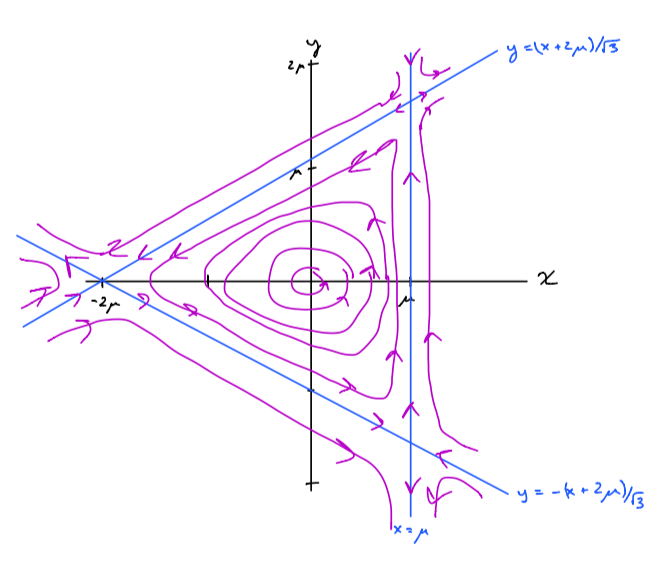
\includegraphics[width=4in]{img/Pset05q1e.png}

% I'll classify the fixed points as well: $f_x = y$, $f_y = x - \mu$, $g_x = \mu + x$, $g_y = -y$.  The trace is $y - y = 0$ and the determinant is $y(-y) - (\mu + x)(x-\mu) = -y^2 - x^2 + \mu^2$. Classifying the fixed points:

% \begin{tabular}{ c | c | c}
% fixed point & determinant \\
% \hline 
% \hline
% $(0,0)$ &  $\mu^2$ & linear center \\
% \hline
% $(-2\mu, 0)$ & $-3\mu^2$ & saddle point \\
% \hline
% $(\mu, \sqrt{3}\mu)$ & $<0$ & saddle point \\
% \hline
% $(\mu, -\sqrt{3}\mu)$ & $< 0$ & saddle point
% \end{tabular}

% For each saddle point, I'll head to Mathematica to find eigenvalues and eigenvectors.

\end{solution}


\part Identify any heteroclinic or homoclinic connections in your system.

\begin{solution}

The invariant lines connect saddle points so the segments of the invariant lines that connect that saddles are heteroclinic orbits.  There are three of these.

\end{solution}

\part Use a numerical tool to create an accurate phase portrait for a particular value of $\mu$.  Include the name of the tool and any code or instructions needed to reproduce your plot.  Also include the invariant lines you found above on your phase portrait.


\begin{solution}

To make the phase portrait, I use StreamPlot in Mathematica.  I added the fixed points to the portrait and made an additional StreamPlot choosing initial conditions right on the heteroclinic connections so that those are visible in the plot.

\begin{verbatim}
f[x_, y_] := y (-\[Mu] + x)
g[x_, y_] := \[Mu] x + (x^2 - y^2)/2
solns = Solve[{f[x, y] == 0, g[x, y] == 0}, {x, y}]
fixed = ListPlot[{x, y} /. solns /. \[Mu] -> 3, AspectRatio -> 1, 
  PlotMarkers -> Graphics[{Black, Thick, Circle[]}, ImageSize -> 10], 
  Ticks -> {{{-3, -\[Mu]}, {3, \[Mu]}}, {{-3, -\[Mu]}, {3, \[Mu]}}}, 
  AxesLabel -> {x, y}, LabelStyle -> Medium, 
  PlotRange -> {{-8, 4}, {-6, 6}}]
val = 7;
sp = StreamPlot[({f[x, y], g[x, y]} /. \[Mu] -> 3), {x, -val, 
    val}, {y, -val, val}, Frame -> False];
sp1 = StreamPlot[({f[x, y], g[x, y]} /. \[Mu] -> 3), {x, -val, 
   val}, {y, -val, val}, 
  StreamPoints -> {{3, 0}, {0, 2 Sqrt[3]}, {0, -2 Sqrt[3]}}];
Show[fixed, sp, sp1]
\end{verbatim}

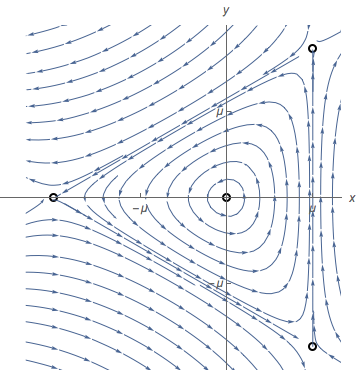
\includegraphics[width=4in]{img/S19pset05p2.png}

\end{solution}

\end{parts}

\question (Projects) This assignment is related to your final project for the course.  It will not be submitted on Gradescope.
\begin{parts}
    \item Choose two of the papers from the Reference list in this problem set, search for those papers, work to read the abstracts, and take a look through the equations, diagrams, and figures in the paper.  
    
    To do the searches, you might use \url{https://scholar.google.com} or another scientific index.  If you use an index beside Google Scholar, mention it in your post.

To access the full text of the paper, go to \url{https://hollis.harvard.edu} and enter the title of the paper in the search bar there.  This is a Harvard library website and will give you online access to the paper if Harvard has a subscription.  If not, it usually has a link for requesting the paper.


Choose one of the two papers, and post to the PSet 05 Q2a Discussion Board on Canvas.  If another student has already posted about the paper, then make your post within the same thread as theirs.  In your post, give the title of the paper, and make a comment about the abstract.  Mention something you found interesting, something you didn't understand, and something else that you would like to share.

\emph{Some of these papers may require building substantial additional knowledge beyond what we are directly studying in the course.}


\item Do a search for a published paper that relates to dynamical systems or bifurcation theory and connects to a topic you are interested in.  Read the abstract to the paper.  
    
Each student should find a unique paper for this, (check the discussion board in Canvas).
    
Search terms related to our course could include \emph{bifurcation, stability, dynamical} etc.

Post to the PSet 05 Q2b Discussion Board on Canvas.  In your post, give the title, authors, and year of the paper.  Share how you found the paper, what led you to choose it, an unfamiliar term that you saw in the abstract or paper, and anything else that you would like to share.

\end{parts}  

  



\textbf{Extra information}

The structure of the final project:

    % \item It can be a dynamical systems modeling project.  In that case, you would work to build a dynamical model (likely a very simple model) with the aim of answering a question you're intrigued by.
 It will be based on a published paper or book chapter.  You will work to understand and replicate key results and will try a small extension or different exploration. % Your contribution requires an act of creative ownership: you might adjust some aspect of the model, shift it to a different context, explore a special case, or anything else you propose.  
 I am providing a list of possible papers for this (\emph{see attached list}), or you can propose a paper.  Only one team per paper.
    % \item It can be learning-oriented with a focus on exploring a dynamical systems topic that is beyond the scope of our course.  In that case, you'll learn about the topic and then will develop materials to guide your classmates or future students in learning about the topic.  A few suggested topics are listed in the ``Exploration Topics'' section.


%We will spend some time in class on \textbf{Friday March 8th} splitting apart by potential interest area so that students with economics / biology / climate / social systems / etc project interests can meet each other.


The default for the project will be to work in a team of three.  If there's a reason that a group of one, two, or four would work better, you'll have a chance to speak with me about arranging an exception. 

The project proposals will be due in late March. %\textbf{Monday, April 1st}.  
A timeline for the project deliverables and more detailed expectations will be included in the next problem set.

% \textbf{Potential exploration topics}
% \begin{itemize}
%     \item pattern formation (Turing bifurcation)
%     \item spatially extended systems
%     \item fast-slow systems
%     \item Melnikov method and routes to chaos
%     \item noise (stochasticity) in dynamical systems
%     \item data assimilation
%     \item control of a dynamical system
%     \item equation-free methods
% \end{itemize}

\nocite{*}
\bibliographystyle{plain}
\bibliography{projects}

% \begin{itemize}
%     \item \textbf{Monday, April 1}: Project proposals due.
%     \begin{itemize}
%         \item If you're basing your project on a paper from the list I've provided, you'll send me a message on Piazza letting me know the paper once you've chosen it, along with the names of your team members, so that I can update the set of available titles.
%     \end{itemize}
%     \item \textbf{Mondays in April}; Project updates.  A project update, along with a team meeting log, an updated reference list, and any simulation code, will be due the 8th, 15th, and 22nd of April.
%     \item \textbf{Friday, April 26}: Peer-editing 1: Presentation.  A draft of your presentation will be due Thursday April 25th.
%     \item \textbf{Monday, April 29 + Wednesday, May 1}: Project presentation 1.
%     \item \textbf{Wednesday, May 1}: Project presentation 1.
%     \item \textbf{Friday, May 3}: Peer-editing 2: 
%     \item \textbf{Saturday, May 11}: Project presentation 2 + Final report.
    
% \end{itemize}

% \noindent The project will consist of two parts: a 10-15 page paper, and a $7$ minute presentation.
%  \vskip.25in

% \noindent
% {\bf The paper:}~(45\% of project grade) The purpose of this part of the project is to practice and refine your written mathematical communication skills that you have been cultivating on homework assignments throughout the semester. This paper should be (roughly) between 10 and 15 pages long, typed in LaTeX, and aimed at an audience of your peers. IMPORTANT: your paper should NOT simply be a rewording or restating of the paper you are studying. You should introduce the background, summarize the authors' key results {\em in your own words}, and then explain your extensions or new results. You should cite any relevant work. You can assume the reader understands everything that we have learned in this class, but you shouldn't assume further mathematical or physical knowledge. Your paper should be in the style of a mathematical document; that is, you should define all new objects you introduce, state and explain models precisely, and give examples. You will be provided with a LaTeX template (link on Piazza) to help you get started. If you are still unclear about what style I am expecting for this document, come talk to me. This document is your magnum opus of the semester. Take time to create something that illustrates your newly obtained knowledge/skillset and is a manuscript you can be proud of. Also - edit this! Several times! Grading rubric is attached.
% \vskip.25in
% \noindent
% {\bf The presentation:}~(45\% of project grade) The purpose of this part of the project is to demonstrate your verbal mathematics communication skills that you have been developing by working with your peers in class. Each group will give a $7$ minute presentation on their project. Groups may decide to have one person give the presentation, or multiple group members may split the presentation time. Be aware that seven minutes is not very long to explain a 10-15 page paper! This means you should practice to make sure you fall within the allotted time. Think carefully about what you are going to say and how you can best express your ideas concisely. You are welcome to use either presentation tools (Powerpoint, Beamer slides, etc.) or just boards. Grading rubric is attached.
% \vskip.25in
% \noindent
% Finally, if you have no idea what to do your project on or who to work with, come talk to me! I'm here to help you and make this a positive experience - please reach out to me if the idea of this project is making you anxious. 



\end{questions}




\end{document}
